% Created 2020-05-29 vie 16:53
% Intended LaTeX compiler: pdflatex
\documentclass[11pt]{article}
\usepackage[utf8]{inputenc}
\usepackage[T1]{fontenc}
\usepackage{graphicx}
\usepackage{grffile}
\usepackage{longtable}
\usepackage{wrapfig}
\usepackage{rotating}
\usepackage[normalem]{ulem}
\usepackage{amsmath}
\usepackage{textcomp}
\usepackage{amssymb}
\usepackage{capt-of}
\usepackage{hyperref}
\usepackage{minted}
\author{Lucas Michel Todó}
\date{31/03/2020}
\title{Creation of active gene-lists}
\hypersetup{
 pdfauthor={Lucas Michel Todó},
 pdftitle={Creation of active gene-lists},
 pdfkeywords={},
 pdfsubject={},
 pdfcreator={Emacs 26.3 (Org mode 9.2)},
 pdflang={English}}
\begin{document}

\maketitle
\tableofcontents \clearpage
\section{Active/Inactive Gene lists}
\label{sec:orgb8ba823}
Our aim is to create a unified table that assigns to each gene in the P.falicparum gnome a expresion state.
We will define 5 possible expresion states:

\begin{itemize}
\item Active
\begin{itemize}
\item Active (no-variant genes)
\item Variant Active
\item Variant Semiactive (vairant genes with an intermediate state)
\end{itemize}

\item Inactive (no-variant genes)
\begin{itemize}
\item Variant Repressed
\end{itemize}

\item Not-Settable
\end{itemize}

\subsection{Microarray Data: Red Signal}
\label{sec:org25656e2}
We willl load the red signal and transform it into percentiles. For each gene we pick the "Aver.2Higher" column from the original microarrays data table. This column corresponds to the average between the two highest red signals among available timepoints.

Red Signal DataFrame
\begin{verbatim}
        Gene_id     Red_12B     Red_10G   Red_3D7B Percent_12B Percent_10G
1    mal_mito_3 22579.33333 36436.73333 30636.8250  96.0466005  98.4721161
2 PF3D7_0100100   104.17083   215.03542   264.4000   5.6913675  10.9625668
3 PF3D7_0100200  1357.70000    72.67917   724.1500  29.7555386   4.0106952
4 PF3D7_0100300   283.98333   291.69583  7540.9042  12.5668449  12.9870130
5 PF3D7_0100400   193.77500    35.01250   161.0833   9.8930481   1.0504202
6 PF3D7_0100600    31.58333    33.40417    31.5250   0.2291826   0.4392666
  Percent_3D7B MaxRedPercentDif MeanRedPercent MaxRedPercent
1   97.8800611         2.425516     97.4662592    98.4721161
2   11.1153552         5.423988      9.2564298    11.1153552
3   19.9006875        25.744843     17.8889738    29.7555386
4   81.3407181        68.773873     35.6315253    81.3407181
5    8.0595875         8.842628      6.3343519     9.8930481
6    0.2387319         0.210084      0.3023937     0.4392666
\end{verbatim}

\subsection{Microarray Data: Areas}
\label{sec:orgf9faa78}
We will load the areas data to calculate FC among strains. For each gene, we select the time interval (right, left, mid or sides) for which we find the maximum difference among strains (between highest and lowest). We will also add a column to check if this time interval corresponds to the interval of maxium expression for each strain.

Areas DataFrame
\begin{verbatim}
              Gene_id     l_12B     r_12B     m_12B    s_12B     l_10G    r_10G
1          mal_mito_3 30.592496 61.080128 49.676556 41.99607 25.372470 62.38873
2 MAL13P1.415_oldname  5.423269  8.488971  1.289779 12.62246  6.117132 10.59524
3  MAL13P1.65_oldname 18.322430        NA 17.593468       NA 14.071128       NA
4  MAL7P1.142_oldname  9.389247 12.807814 10.340803 11.85626 13.661078 14.52676
5  MAL8P1.310_oldname        NA        NA        NA       NA        NA       NA
6   MAL8P1.90_oldname        NA        NA        NA       NA        NA       NA
      m_10G    s_10G    l_3D7B   r_3D7B    m_3D7B    s_3D7B   MaxLeft   MinLeft
1 49.805504 37.95570 25.484634 62.83441 50.462696 37.856349 30.592496 25.372470
2  3.676218 13.03616  1.789873 10.51234  3.691753  8.610459  6.117132  1.789873
3        NA       NA 19.333324       NA        NA        NA 19.333324 14.071128
4 13.401610 14.78623  7.099032 13.34518 12.041177  8.403034 13.661078  7.099032
5        NA       NA        NA       NA        NA        NA        NA        NA
6        NA       NA        NA       NA        NA        NA        NA        NA
  MaxRight  MinRight    MaxMid    MinMid MaxSides  MinSides  DifLeft DifRight
1 62.83441 61.080128 50.462696 49.676556 41.99607 37.856349 5.220025 1.754283
2 10.59524  8.488971  3.691753  1.289779 13.03616  8.610459 4.327259 2.106274
3       NA        NA        NA        NA       NA        NA 5.262196       NA
4 14.52676 12.807814 13.401610 10.340803 14.78623  8.403034 6.562046 1.718950
5       NA        NA        NA        NA       NA        NA       NA       NA
6       NA        NA        NA        NA       NA        NA       NA       NA
     DifMid DifSides Interval   MaxDif    areaFC  area_12B area_10G area_3D7B
1 0.7861401 4.139719     Left 5.220025 0.3881060 30.592496 25.37247 25.484634
2 2.4019733 4.425700    Sides 4.425700 0.3290483 12.622460 13.03616  8.610459
3        NA       NA     Left 5.262196 0.3912413 18.322430 14.07113 19.333324
4 3.0608067 6.383199     Left 6.562046 0.4878845  9.389247 13.66108  7.099032
5        NA       NA  No Data       NA        NA        NA       NA        NA
6        NA       NA  No Data       NA        NA        NA       NA        NA
   MaxArea   MinArea
1 30.59250 25.372470
2 13.03616  8.610459
3 19.33332 14.071128
4 13.66108  7.099032
5       NA        NA
6       NA        NA
\end{verbatim}

\subsection{Load RNA-Seq Data}
\label{sec:orge943a5f}
We will use publicly available data from PlasmoDB to create a reference expresion percentile for each gene.
All data-sets are from RNA-Seq studies in the 3D7 strain.
We are using 4 different data-sets:
\begin{itemize}
\item Otto et.al.
\item Hoeijmakers et.al.
\item Toenhake et.al.
\item Bartfai et.al.
\end{itemize}

We use only uniquely mapped reads and scaled data when available.
For each Data-Set we first create a column representing the maxium value among timepoints for each gene. We then convert this column into percentile values. Finally we average this percentile values among all Data-Sets.


RNA-Seq DataFrame
\begin{verbatim}
        Gene_id Otto_Max_pcnt Hoeij_Max_pcnt Toen_Max_pcnt Bart_Max_pcnt
1    mal_mito_1     97.695933      66.259382      69.20929     80.520161
2    mal_mito_2     98.079944      88.776401      85.12829     94.728574
3    mal_mito_3     97.835573      92.249956      89.99825     90.190260
4 PF3D7_0100100     26.104032      24.855996      17.57724     18.240531
5 PF3D7_0100200      7.366032      25.693838      13.83313     18.764182
6 PF3D7_0100300     22.045732       3.587013       2.46989      1.885146
  MeanPercent StdDevPercent
1   78.421190     12.335823
2   91.678303      5.040060
3   92.568511      3.166454
4   21.694449      3.818402
5   16.414296      6.711285
6    7.496945      8.421970
\end{verbatim}

We plot the resulting distribution of percentiles (it should be almost flat).
\begin{center}
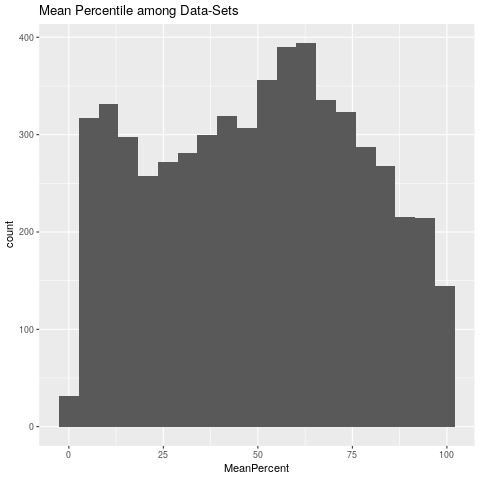
\includegraphics[width=.9\linewidth]{./Plots/rnaseq_perc.png}
\end{center}


We plot the standard deviation of the percentile values among different Data-Sets and we can see that for the vast majority of genes it doesn't go above 10.
\begin{center}
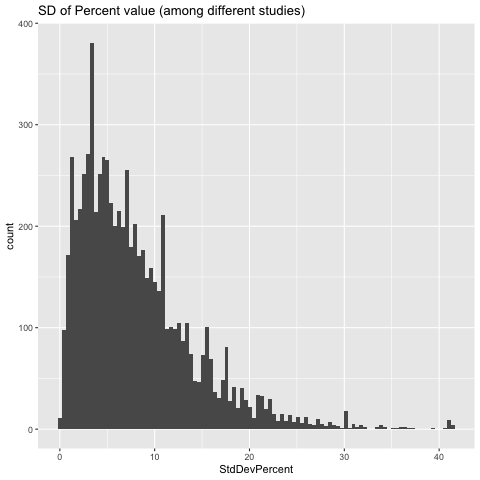
\includegraphics[width=.9\linewidth]{./Plots/rnaseq_perc_sd.png}
\end{center}
\subsection{Create table for classification}
\label{sec:org01967d0}

Joining and summarizing all the prevoius data we create a a table that will let us classify the genes according to their expression state.

To classify genes, we add a colum for each strain were we classify genes according to their expression relative to other strains.
To create this column we have taken the maximum and minimum area value for each gene and divided this interval in 3 equal regions. Each strain then gets a value of man/mid/max according to which region it falls.

\texttt{gene-min-{}--{}-|-{}--mid-{}--{}-|-{}--{}-gene-max}

Final DataFrame
\begin{verbatim}

        Gene_id Variant Percent_12B Percent_10G Percent_3D7B MaxRedPercentDif
1    mal_mito_3   FALSE  96.0466005  98.4721161   97.8800611         2.425516
2 PF3D7_0100100    TRUE   5.6913675  10.9625668   11.1153552         5.423988
3 PF3D7_0100200    TRUE  29.7555386   4.0106952   19.9006875        25.744843
4 PF3D7_0100300    TRUE  12.5668449  12.9870130   81.3407181        68.773873
5 PF3D7_0100400    TRUE   9.8930481   1.0504202    8.0595875         8.842628
6 PF3D7_0100600    TRUE   0.2291826   0.4392666    0.2387319         0.210084
  MeanRedPercent MaxRedPercent Interval    areaFC area_12B  area_10G area_3D7B
1     97.4662592    98.4721161     Left 0.3881060 30.59250 25.372470  25.48463
2      9.2564298    11.1153552     Left 0.8879945 31.76998 43.713503  38.29839
3     17.8889738    29.7555386    Right 3.5015562 52.33320  5.237266  43.02460
4     35.6315253    81.3407181     Left 3.3957657 31.78908 33.073957  77.46213
5      6.3343519     9.8930481     Left 2.0671154 23.21846  7.706832  35.50954
6      0.3023937     0.4392666  No Data        NA       NA        NA        NA
   MaxArea   MinArea MeanPercent rel_12B rel_10G rel_3D7B Gene_name
1 30.59250 25.372470   92.568511     max     min      min      null
2 43.71350 31.769976   21.694449     min     max      mid       VAR
3 52.33320  5.237266   16.414296     max     min      max       RIF
4 77.46213 31.789080    7.496945     min     min      max       VAR
5 35.50954  7.706832   14.607698     mid     min      max       RIF
6       NA        NA    4.789230      NA      NA       NA       RIF
                                   Annot
1                    unspecified product
2 erythrocyte membrane protein 1, PfEMP1
3                                  rifin
4 erythrocyte membrane protein 1, PfEMP1
5                                  rifin
6                                  rifin
\end{verbatim}

\subsection{Create Lists according to thresholds}
\label{sec:org4ed0248}

Now that we have all the data loaded in, we can star to set labels for each gene.

We have set the following thresholds:
\begin{itemize}
\item (rna\_pcnt) RNA-Seq mean percentile: 25\%
\item (red\_pcnt) Red Signal Percentile (by sample): 25\%
\item (red\_rescue) Red Signal Mean Percentile for "rescuing": 40\%
\item (area\_fc) Area log2 Fold-Change: 1
\end{itemize}

In addition to these thresholds we will use 2 more columns to set the categories:
\begin{itemize}
\item Variant: a column stating if gene is variant/non-variant
\item Relative Expression (by strain): a colum were each gene is set to min/mid/max according to it's expression level relative to the other strains.
\end{itemize}

We will have the following categories with the following logic:

\begin{center}
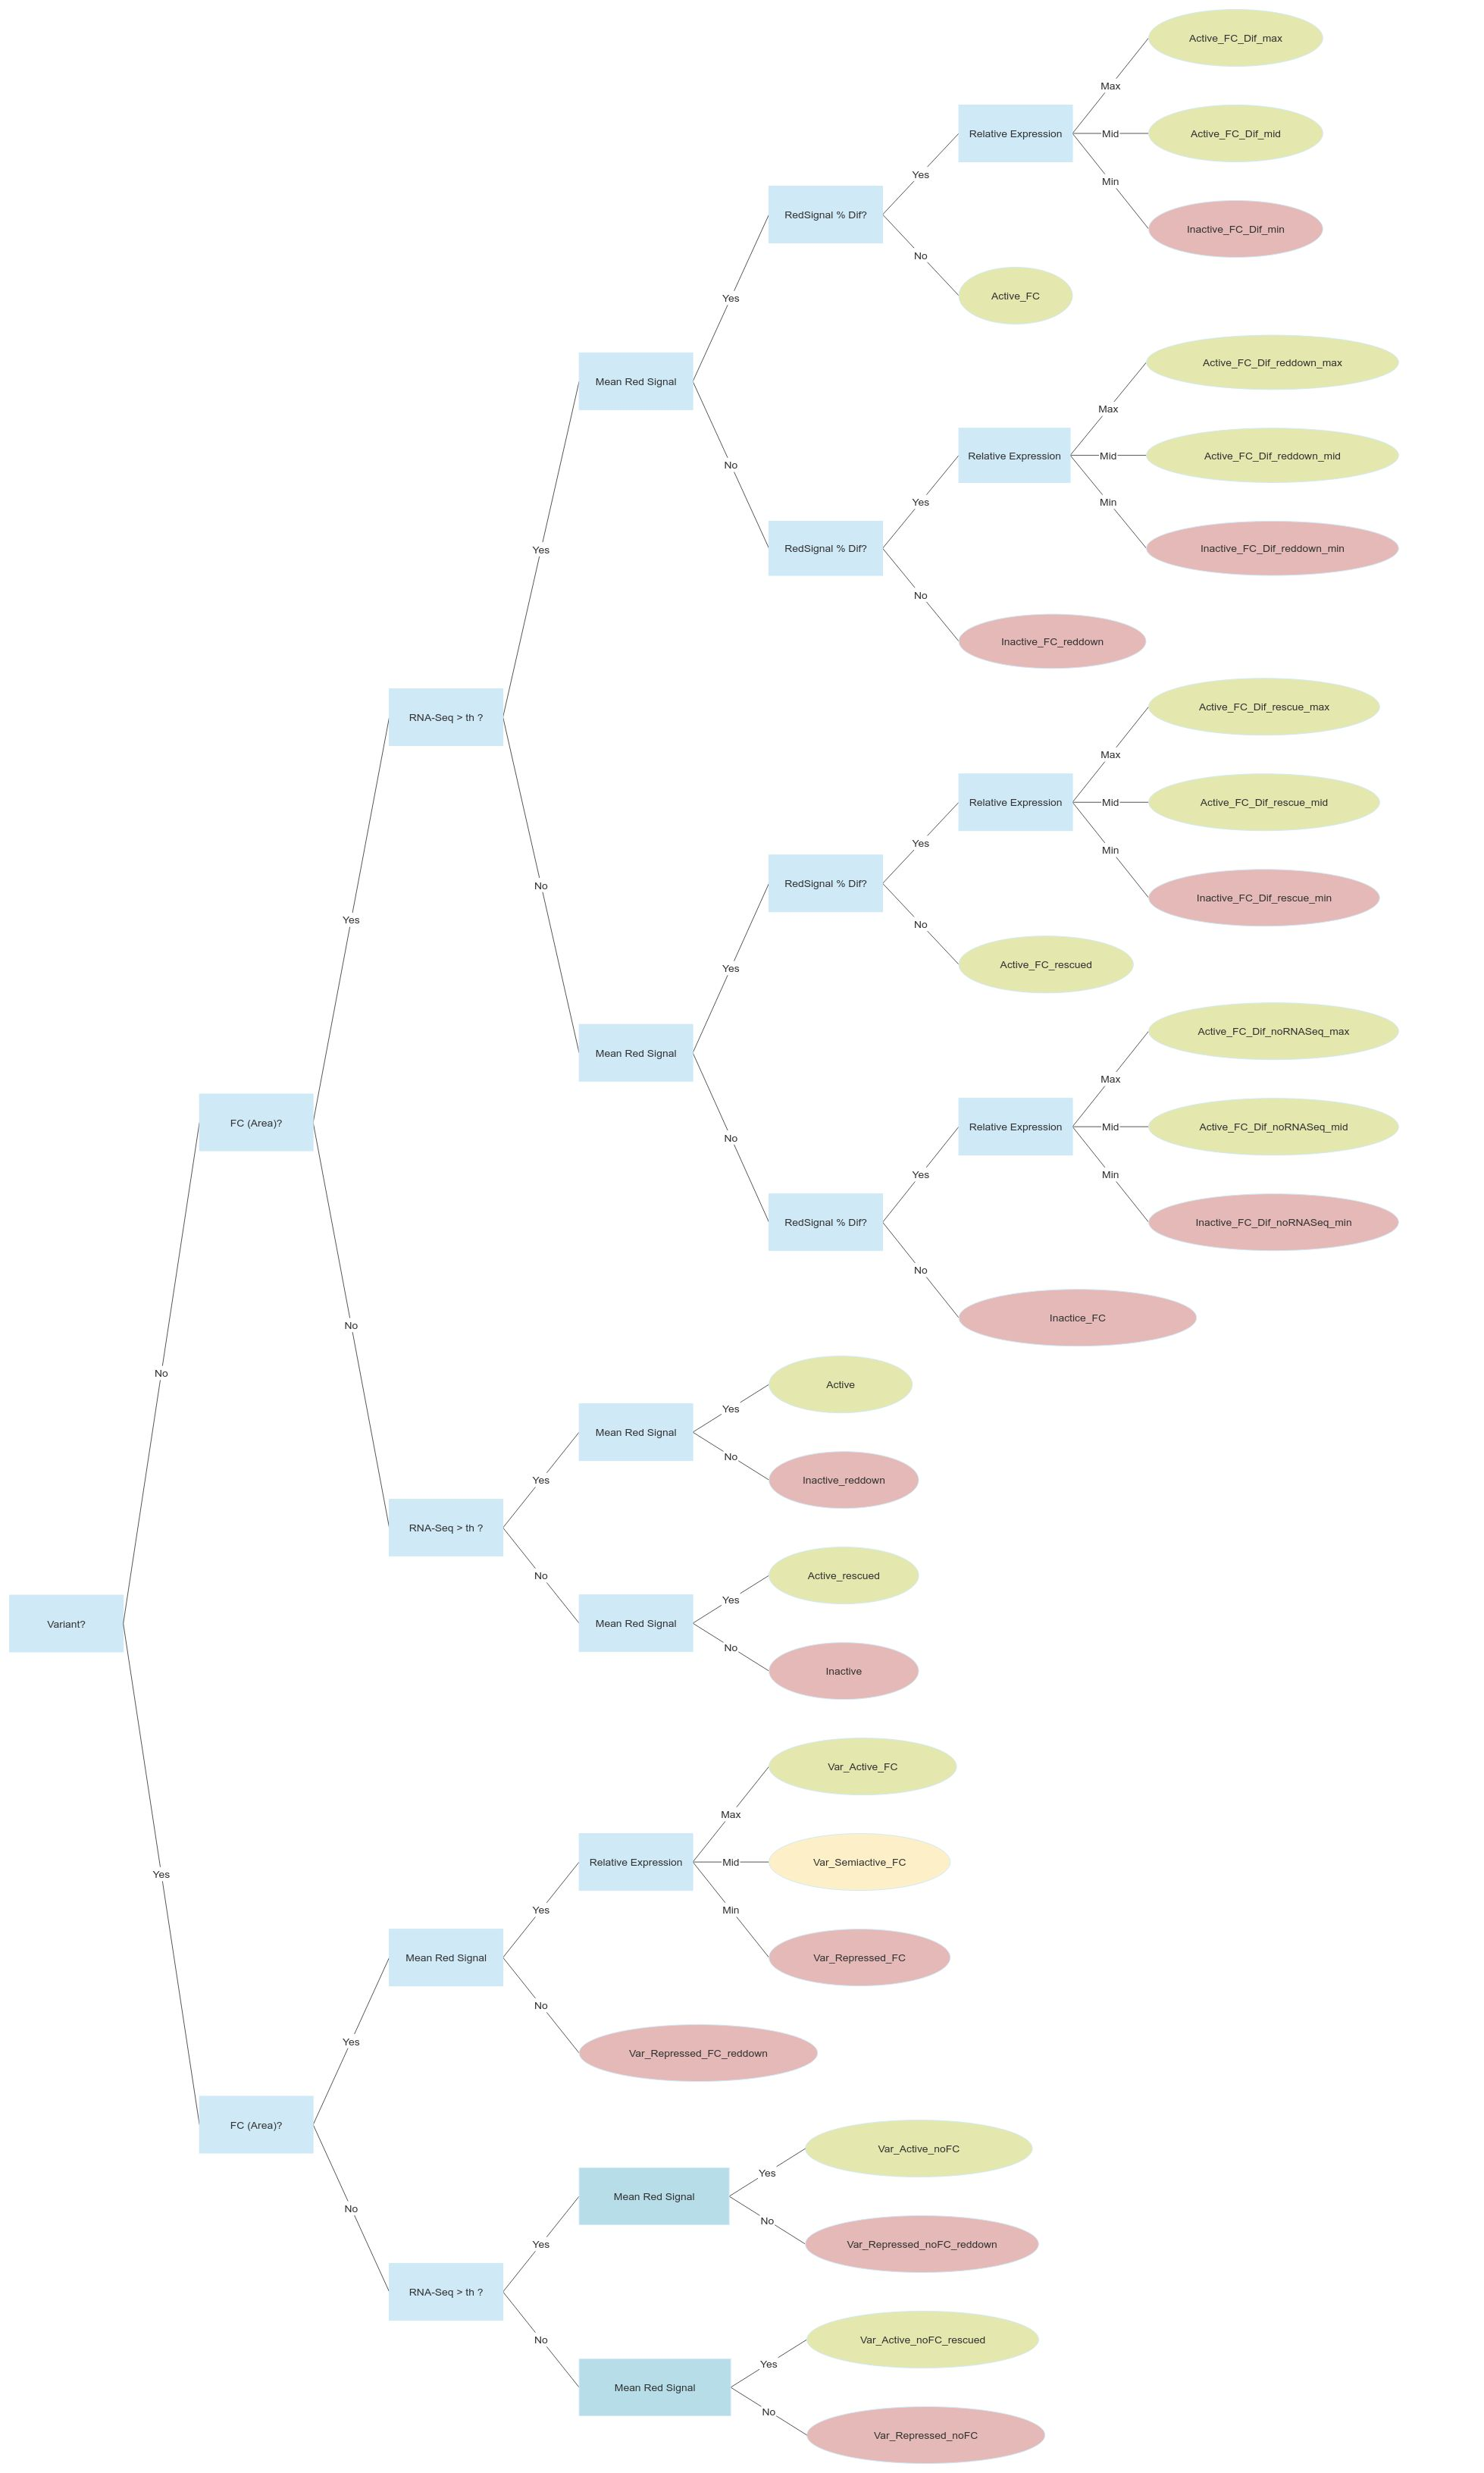
\includegraphics[width=.9\linewidth]{./Plots/Decision_Tree.jpg}
\end{center}

\href{./Plots/Decision\_Tree.jpg}{Make bigger}


Genes that have NA values in any of the classification columns are classified according to the following tree.
\begin{center}
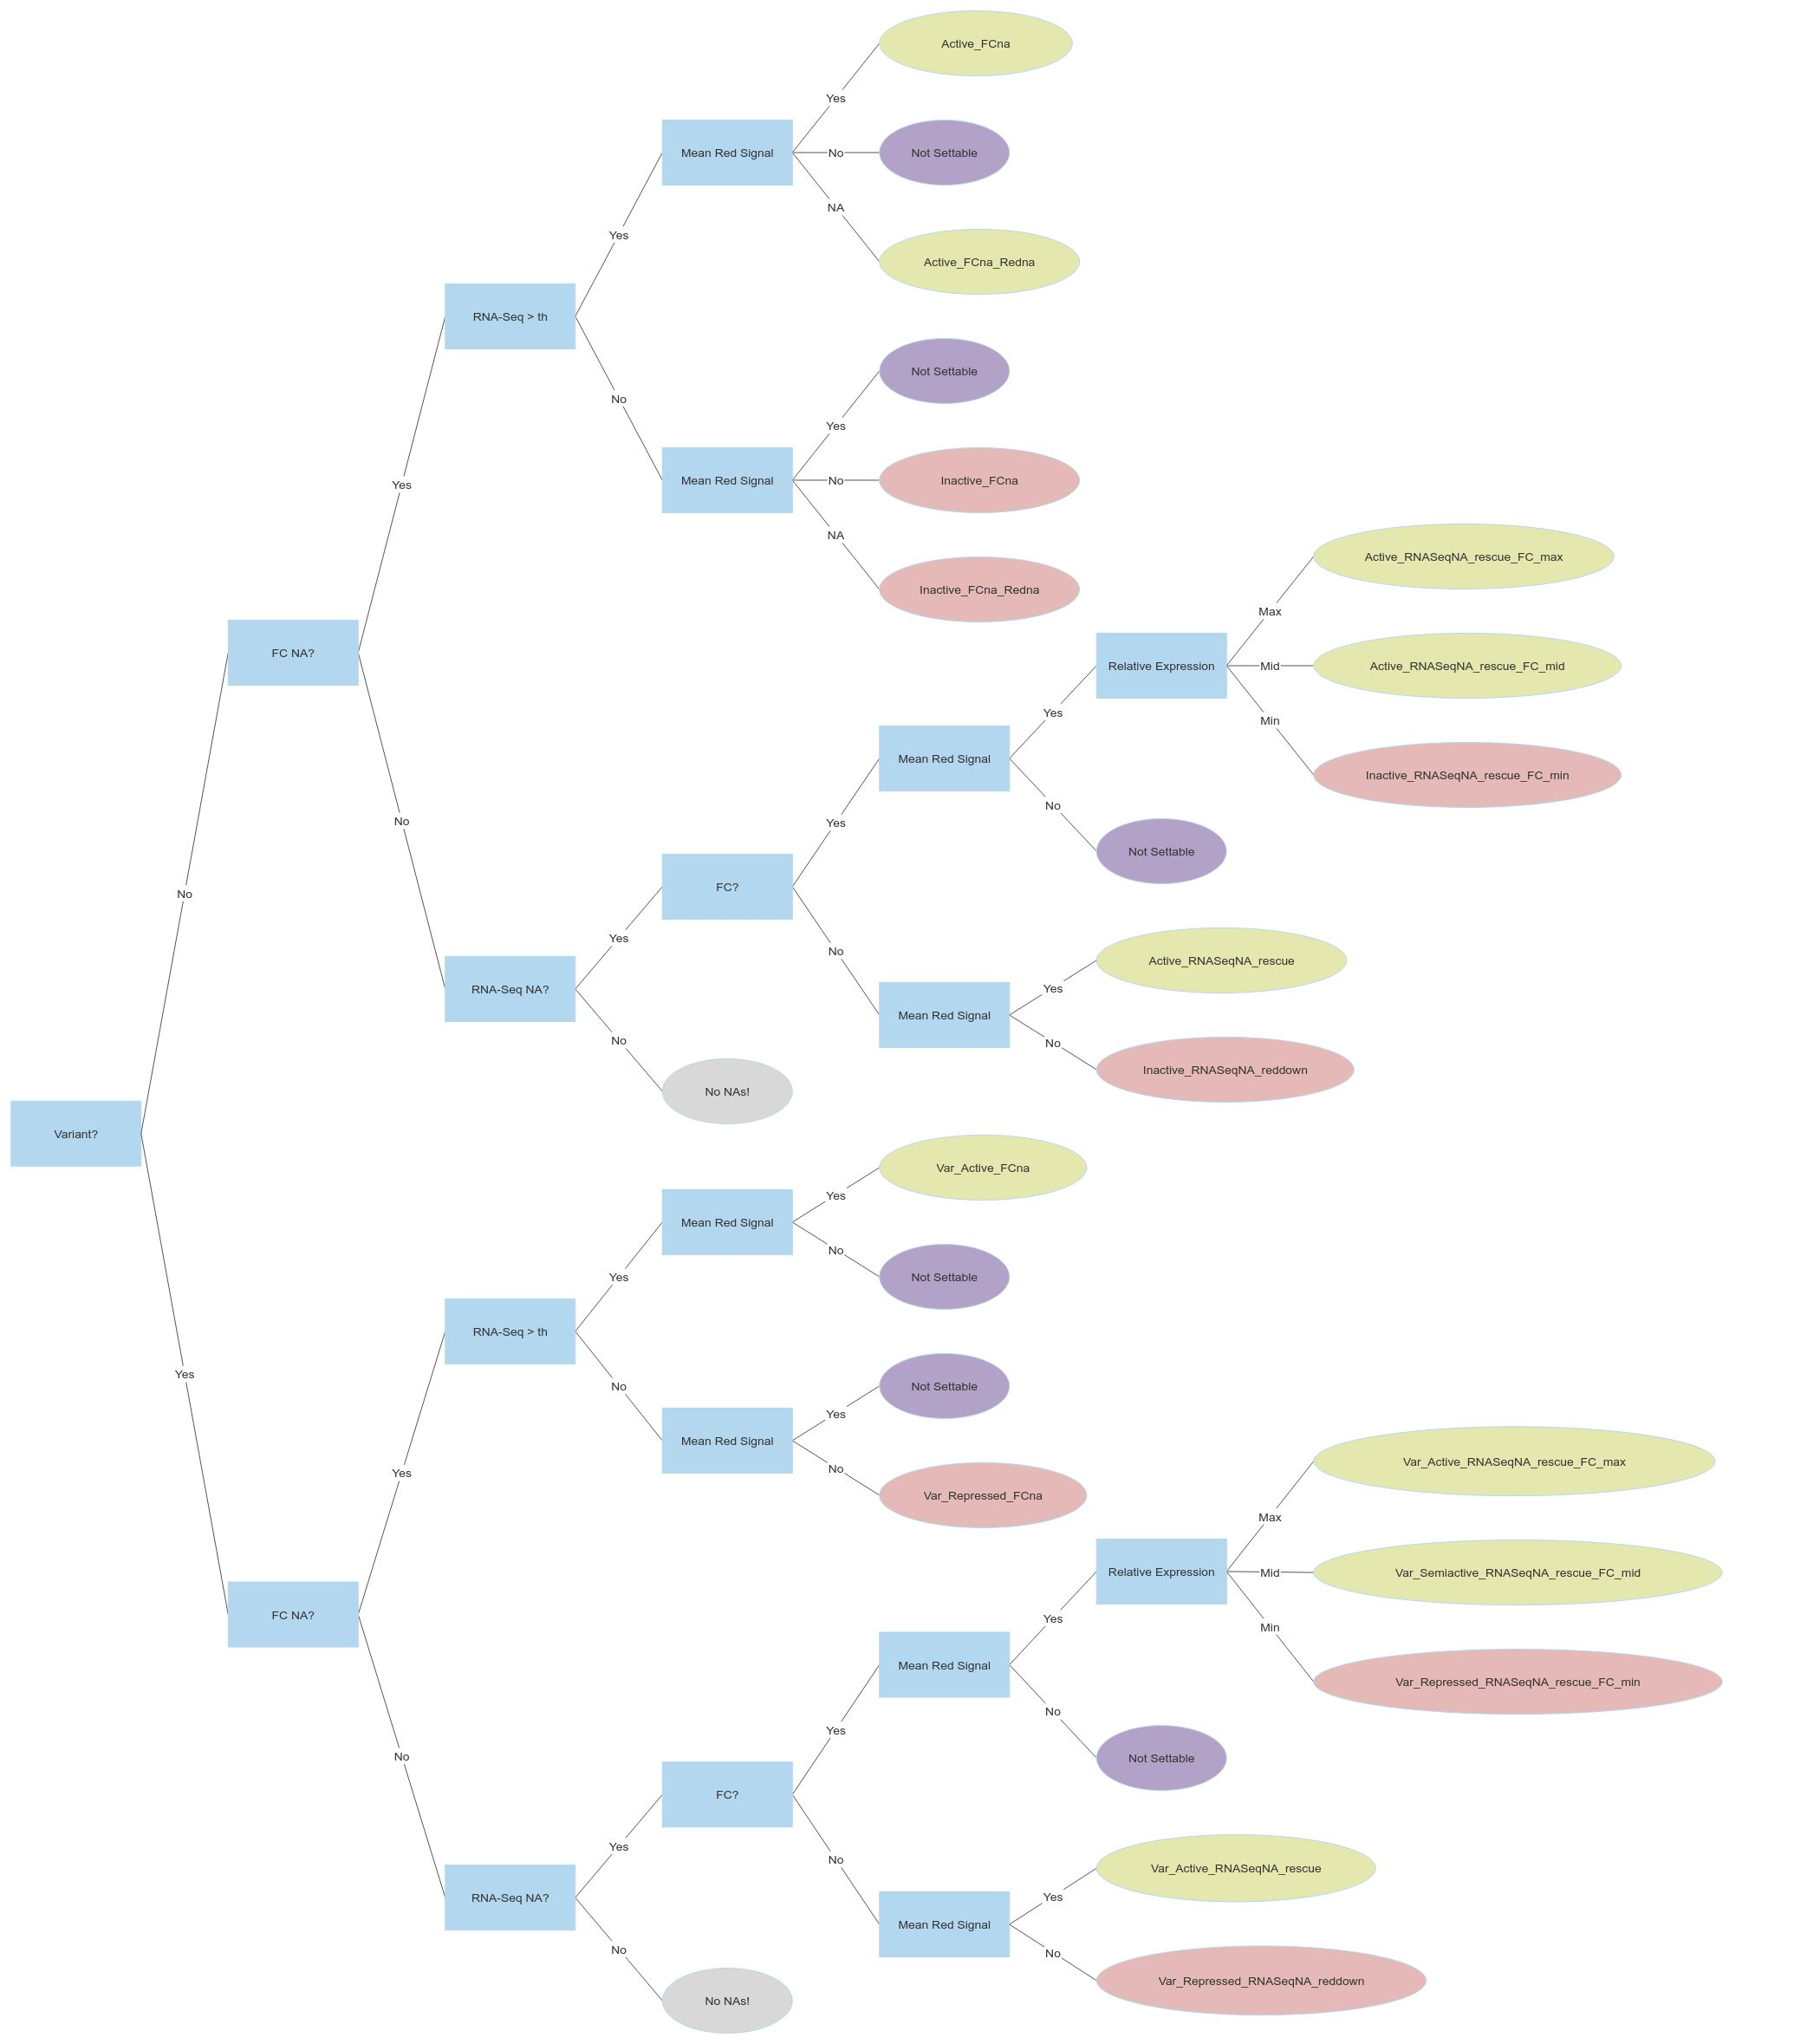
\includegraphics[width=.9\linewidth]{./Plots/active_genes_NAs.jpg}
\end{center}

\href{Plots/active\_genes\_NAs.jpg}{Make bigger}

Using this criteria we construct the following DataFrame:

Gene-State DataFrame
\begin{verbatim}

        Gene_id Variant Percent_12B Percent_10G Percent_3D7B MaxRedPercentDif
1    mal_mito_3   FALSE  96.0466005  98.4721161   97.8800611         2.425516
2 PF3D7_0100100    TRUE   5.6913675  10.9625668   11.1153552         5.423988
3 PF3D7_0100200    TRUE  29.7555386   4.0106952   19.9006875        25.744843
4 PF3D7_0100300    TRUE  12.5668449  12.9870130   81.3407181        68.773873
5 PF3D7_0100400    TRUE   9.8930481   1.0504202    8.0595875         8.842628
6 PF3D7_0100600    TRUE   0.2291826   0.4392666    0.2387319         0.210084
  MeanRedPercent MaxRedPercent Interval    areaFC area_12B  area_10G area_3D7B
1     97.4662592    98.4721161     Left 0.3881060 30.59250 25.372470  25.48463
2      9.2564298    11.1153552     Left 0.8879945 31.76998 43.713503  38.29839
3     17.8889738    29.7555386    Right 3.5015562 52.33320  5.237266  43.02460
4     35.6315253    81.3407181     Left 3.3957657 31.78908 33.073957  77.46213
5      6.3343519     9.8930481     Left 2.0671154 23.21846  7.706832  35.50954
6      0.3023937     0.4392666  No Data        NA       NA        NA        NA
   MaxArea   MinArea MeanPercent rel_12B rel_10G rel_3D7B Gene_name
1 30.59250 25.372470   92.568511     max     min      min      null
2 43.71350 31.769976   21.694449     min     max      mid       VAR
3 52.33320  5.237266   16.414296     max     min      max       RIF
4 77.46213 31.789080    7.496945     min     min      max       VAR
5 35.50954  7.706832   14.607698     mid     min      max       RIF
6       NA        NA    4.789230      NA      NA       NA       RIF
                                   Annot                  state_12B
1                    unspecified product                     Active
2 erythrocyte membrane protein 1, PfEMP1         Var_Repressed_noFC
3                                  rifin              Var_Active_FC
4 erythrocyte membrane protein 1, PfEMP1 Var_Repressed_FC_noredpcnt
5                                  rifin Var_Repressed_FC_noredpcnt
6                                  rifin         Var_Repressed_FCna
                   state_10G                 state_3D7B  category_12B
1                     Active                     Active        Active
2         Var_Repressed_noFC         Var_Repressed_noFC Var_Repressed
3 Var_Repressed_FC_noredpcnt Var_Repressed_FC_noredpcnt    Var_Active
4 Var_Repressed_FC_noredpcnt              Var_Active_FC Var_Repressed
5 Var_Repressed_FC_noredpcnt Var_Repressed_FC_noredpcnt Var_Repressed
6         Var_Repressed_FCna         Var_Repressed_FCna Var_Repressed
   category_10G category_3D7B
1        Active        Active
2 Var_Repressed Var_Repressed
3 Var_Repressed Var_Repressed
4 Var_Repressed    Var_Active
5 Var_Repressed Var_Repressed
6 Var_Repressed Var_Repressed
\end{verbatim}

\subsection{Some results}
\label{sec:org2d1ca63}
This is a table with the number of genes in each state for each strain.

States Table
\begin{verbatim}
  Strain Active Active_FC Active_FC_Dif_max Active_FCna Active_FCna_Redna
1    12B   3944        20                 2           1               191
2    10G   3944        20                 2           1               191
3   3D7B   3944        20                 2           1               191
  Active_rescued Active_RNASeqNA_rescue Inactive Inactive_FC
1             53                      6      660          36
2             53                      6      660          36
3             53                      6      660          36
  Inactive_FC_Dif_min Inactive_FC_reddown Inactive_FCna Inactive_FCna_Redna
1                   2                   5            30                  89
2                   2                   5            30                  89
3                   2                   5            30                  89
  Inactive_reddown Not_Settable Var_Active_FC Var_Active_noFC
1               36          152             8              52
2               36          152             7              52
3               36          152            58              52
  Var_Active_noFC_rescued Var_Active_RNASeqNA_rescue Var_Repressed_FC
1                       3                          1                7
2                       3                          1                5
3                       3                          1                3
  Var_Repressed_FC_noredpcnt Var_Repressed_FCna Var_Repressed_noFC
1                        137                 92                128
2                        141                 92                128
3                         92                 92                128
  Var_Repressed_noFC_reddown Var_Semiactive_FC
1                          4                 1
2                          4                NA
3                          4                NA
\end{verbatim}

And this are the Clag genes
\begin{verbatim}
        Gene_id Variant Percent_12B Percent_10G Percent_3D7B MaxRedPercentDif
1 PF3D7_0302200    TRUE    78.68602    99.57983     42.32238         57.25745
2 PF3D7_0302500    TRUE    98.81589    84.39649     98.98778         14.59129
  MeanRedPercent MaxRedPercent Interval   areaFC  area_12B area_10G area_3D7B
1       73.52941      99.57983    Right 4.823089  37.32948 88.19577  23.32522
2       94.06672      98.98778    Right 3.452270 100.12065 53.68762  99.58767
    MaxArea  MinArea MeanPercent rel_12B rel_10G rel_3D7B Gene_name
1  88.19577 23.32522    76.36804     min     max      min   CLAG3.2
2 100.12065 53.68762    88.72404     max     min      max   CLAG3.1
                                     Annot        state_12B        state_10G
1 cytoadherence linked asexual protein 3.2 Var_Repressed_FC    Var_Active_FC
2 cytoadherence linked asexual protein 3.1    Var_Active_FC Var_Repressed_FC
        state_3D7B  category_12B  category_10G category_3D7B
1 Var_Repressed_FC Var_Repressed    Var_Active Var_Repressed
2    Var_Active_FC    Var_Active Var_Repressed    Var_Active
\end{verbatim}

\subsection{Venn Diagrams}
\label{sec:orgde82d5d}
Here we plon Venn diagrams to visualize how the strains compare.

First we check how many genes share the same "state" among strains:

\begin{center}
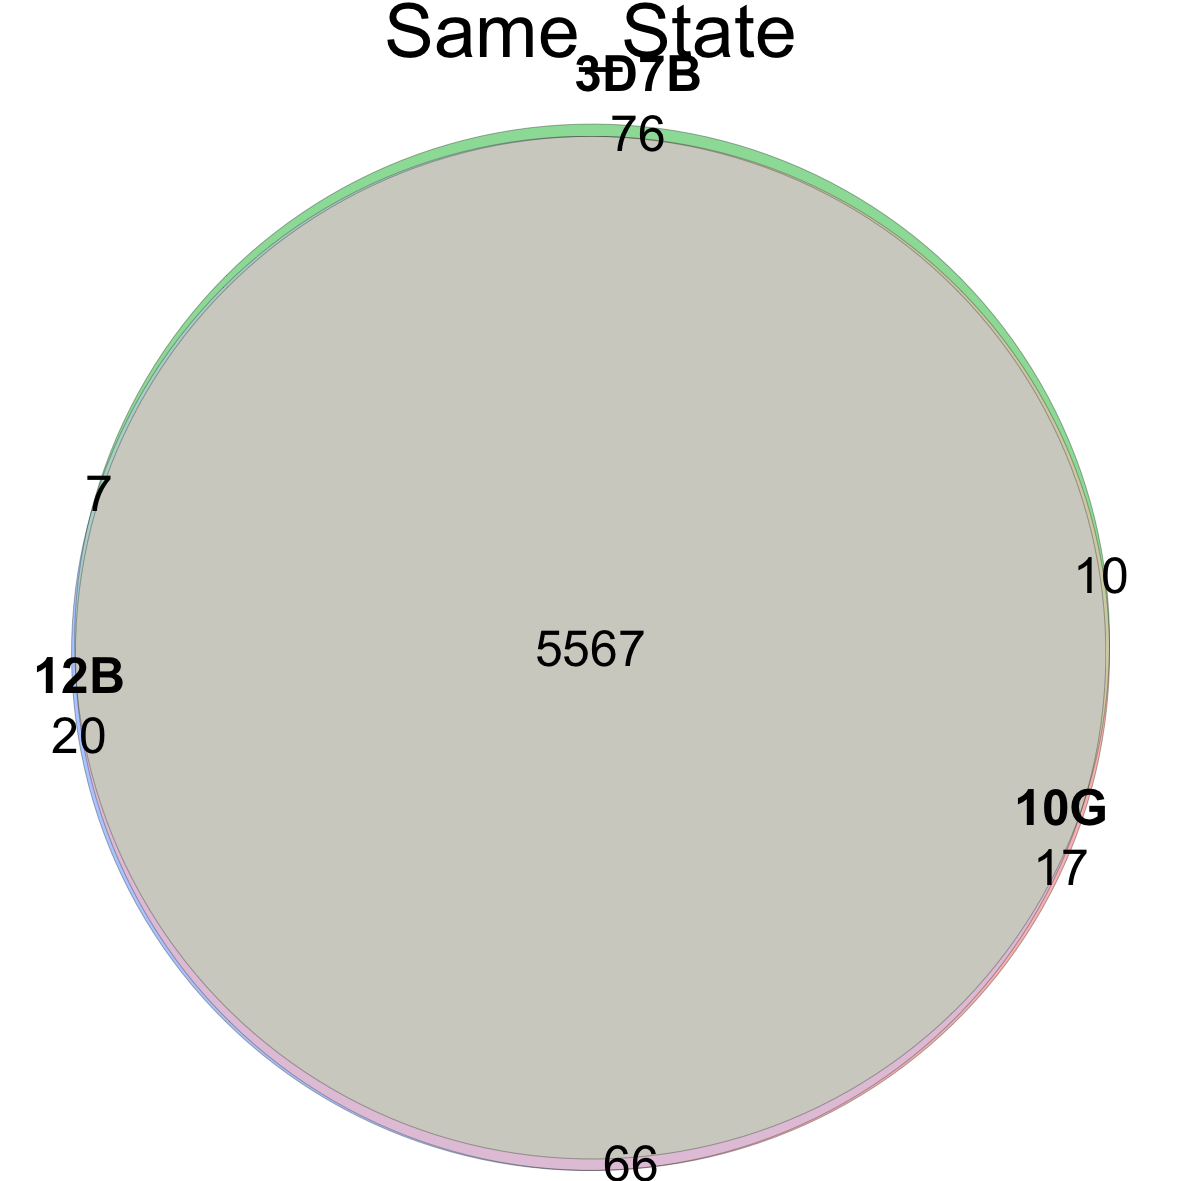
\includegraphics[width=.9\linewidth]{./Plots/venn_Same_State.png}
\end{center}

Then we make venn diagrams for the "Var\_active" and "Var\_Repressed" states.

\begin{center}
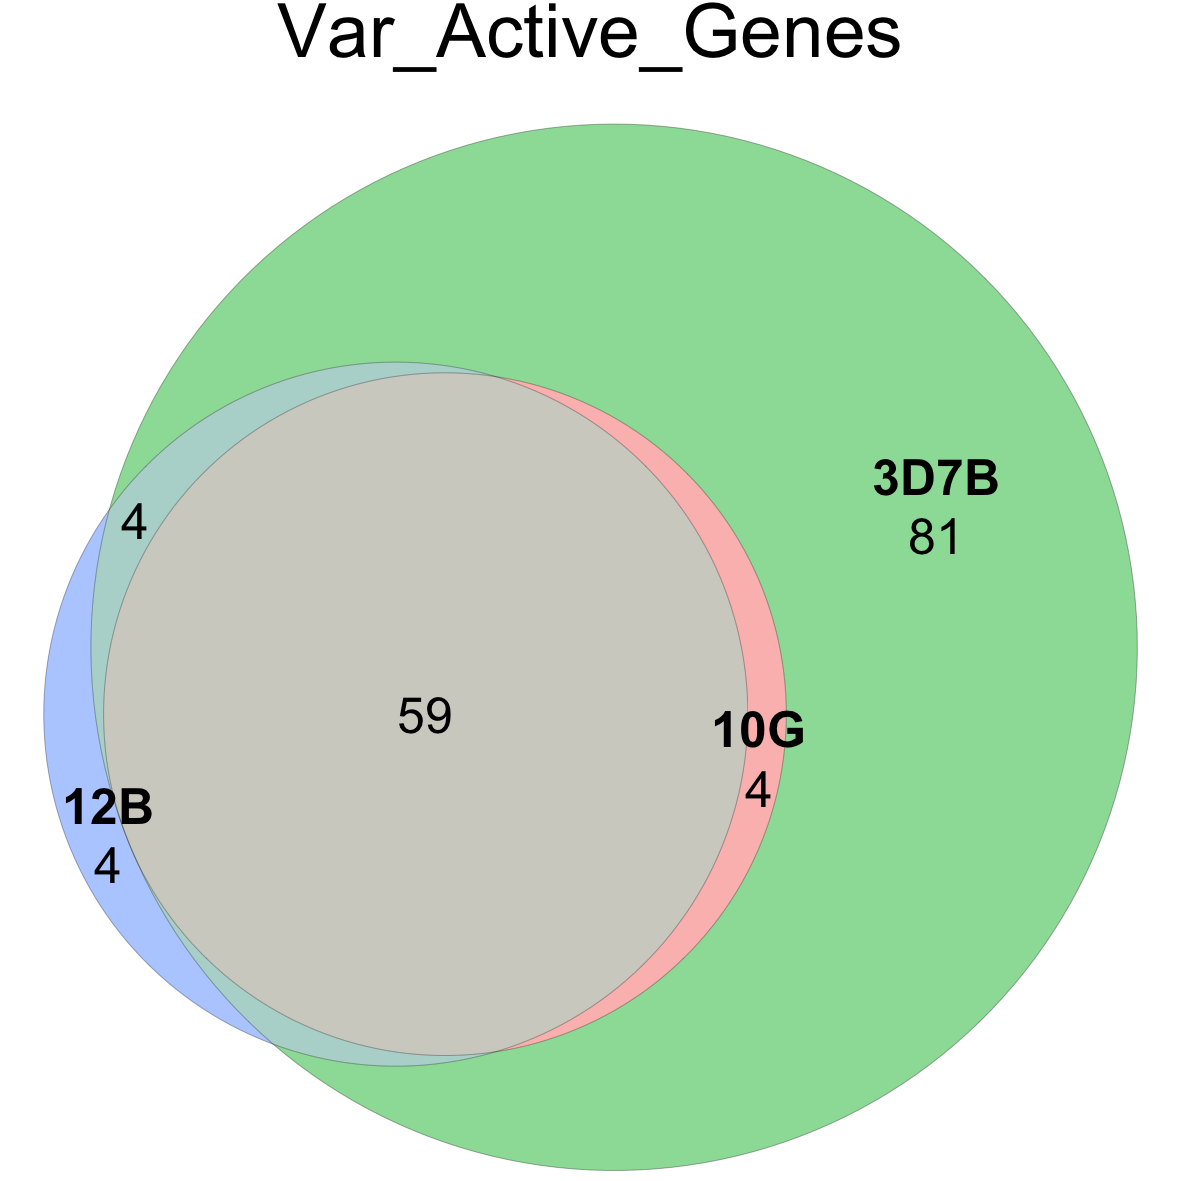
\includegraphics[width=.9\linewidth]{./Plots/venn_Var_Active_Genes.png}
\end{center}

\begin{center}
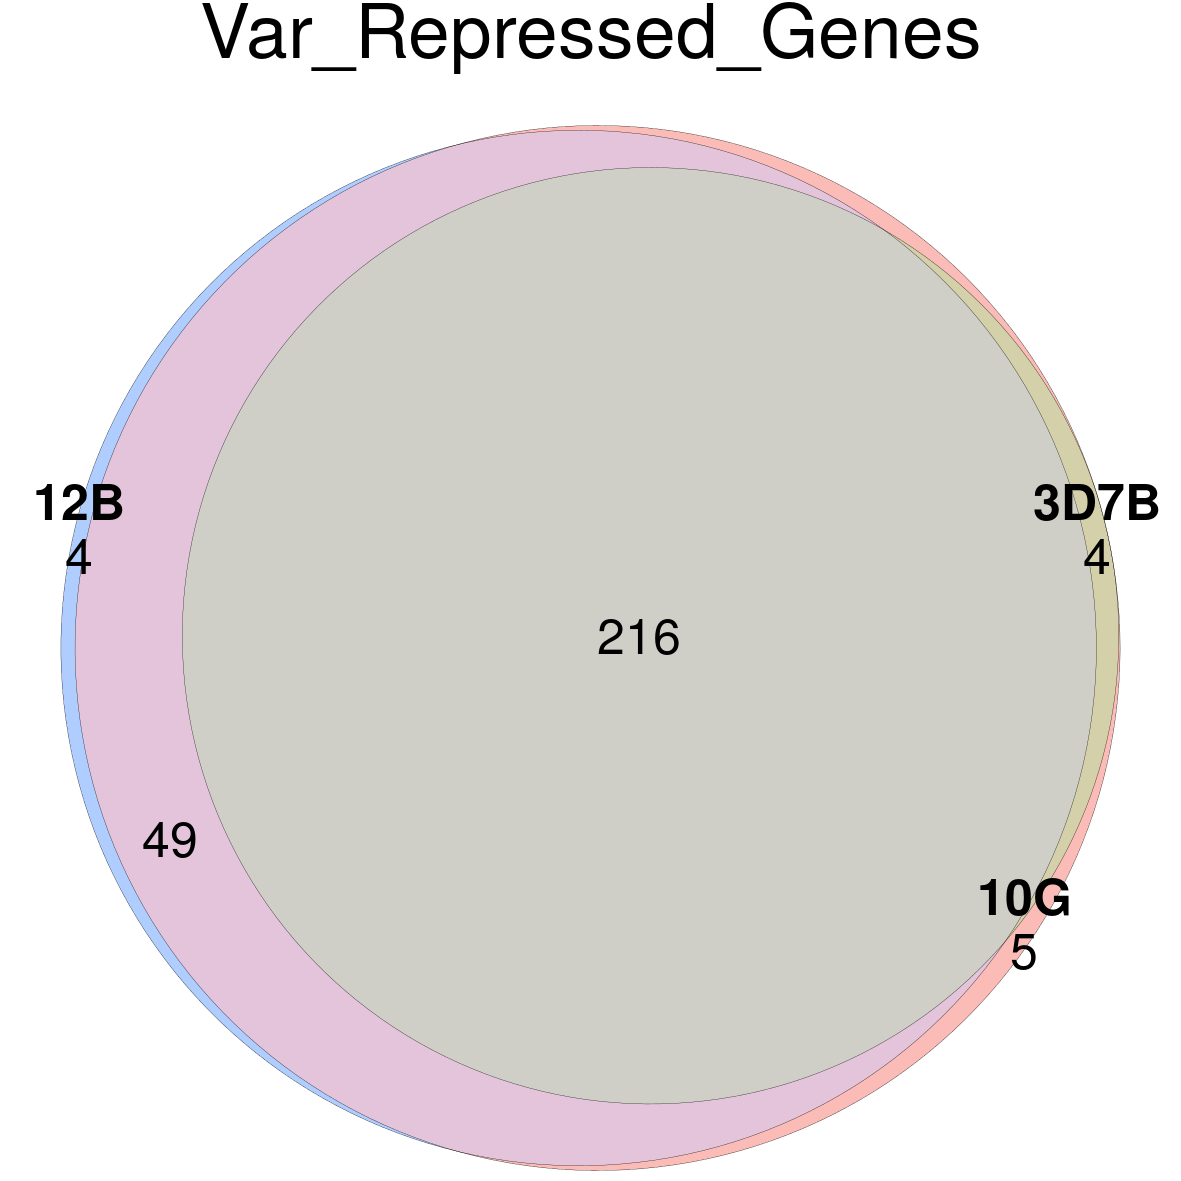
\includegraphics[width=.9\linewidth]{./Plots/venn_Var_Repressed_Genes.png}
\end{center}

\section{Code}
\label{sec:org862a98b}
\subsection{Load Packages and functions}
\label{sec:org6f0fca3}
\begin{minted}[]{r}
#### Imports ####

library(readxl)
library(tidyverse)
library(eulerr)

#### Max Dif function ####

max_dif <- function(vect){
  mx <- max(vect, na.rm = T)
  mn <- min(vect, na.rm = T)
  if (is.infinite(mx) | is.infinite(mn)) {
    md <- NA
  } else {
    md <- mx - mn
  }
  return(md)
}
\end{minted}

\subsection{Microarray Data: Red Signal}
\label{sec:org74fa92d}

\begin{minted}[]{r}
#### Red Signal DF ####

## Read translation table
map <- read.csv('./Data/oldnames_table.csv', stringsAsFactors = F)
excl <- "./Data/3D7_Variantome_AllData_withGam.xls"

## Import Red Signal table
red <- read_excel(excl, sheet = 4)

colnames(red)[1] <- "Old_id"

red_df <- red %>%
  select(Old_id,
         Red_12B = `Aver.2Higher1.2B.`,
         Red_10G = `Aver.2Higher10G.`,
         Red_3D7B = `Aver.2Higher3D7-B.`) %>%
  left_join(map, by='Old_id')

## Manually add gene ids that do not appear on map (we blasted the probes to assign them)
red_df <- red_df %>%
  mutate(Gene_id = ifelse(Old_id == 'MAL8P1.310', 'PF3D7_0830200', Gene_id)) %>%
  mutate(Gene_id = ifelse(Old_id == 'PFI0905W', 'PF3D7_0918500', Gene_id)) %>%
  mutate(Gene_id = ifelse(Old_id == 'PFL1580W', 'PF3D7_1232700', Gene_id))

## Collapse gene ids that appear more than once (mean expression)
red_df <- red_df %>%
  select(-Old_id) %>%
  group_by(Gene_id) %>% summarize_all(list(mean))

## Filter out rows with untranslated gene ids (marked by '_oldname')
red_df <- red_df %>%
  filter(!grepl('_oldname', Gene_id))

## Transform into percentiles

red_df <- red_df %>%
  mutate(Percent_12B = (rank(Red_12B)/length(Red_12B))*100) %>%
  mutate(Percent_10G = (rank(Red_10G)/length(Red_10G))*100) %>%
  mutate(Percent_3D7B = (rank(Red_3D7B)/length(Red_3D7B))*100)

## Add max percentile dif

red_df <- red_df %>%
  mutate(MaxRedPercentDif= apply(select(., contains('Percent_')), 1, max_dif)) %>%
  mutate(MeanRedPercent = apply(select(., contains('Percent_')), 1, mean)) %>%
  mutate(MaxRedPercent = apply(select(., contains('Percent_')), 1, max))

print(red_df, width = 200)
hist(red_df$MeanRedPercent)
\end{minted}
\subsection{Microarray Data: Areas}
\label{sec:orgf685e88}
\begin{minted}[]{r}
#### Areas DF ####

# Import Areas table

area <- read_excel(excl, sheet = 2)

colnames(area)[1] <- "Old_id"

area_df <- area %>%
  select(Old_id,
         l_12B = `left.1.2b`,
         r_12B = `right.1.2b`,
         m_12B = `mid.1.2b`,
         s_12B = `sides.1.2b`,
         l_10G = `left.10g`,
         r_10G = `right.10g`,
         m_10G = `mid.10g`,
         s_10G = `sides.10g`,
         l_3D7B = `left.3d7b`,
         r_3D7B = `right.3d7b`,
         m_3D7B = `mid.3d7b`,
         s_3D7B = `sides.3d7b`) %>%

  mutate_at(vars(-Old_id), as.numeric) %>%


  left_join(map, by='Old_id') %>%
  select(-Old_id) %>%
  group_by(Gene_id) %>% summarize_all(list(mean))


print(area_df, width = 200)

area_df <- area_df %>%
  mutate(MaxLeft = apply(select(., contains('l_')), 1, max)) %>%
  mutate(MinLeft = apply(select(., contains('l_')), 1, min)) %>%

  mutate(MaxRight = apply(select(., contains('r_')), 1, max)) %>%
  mutate(MinRight = apply(select(., contains('r_')), 1, min)) %>%

  mutate(MaxMid = apply(select(., contains('m_')), 1, max)) %>%
  mutate(MinMid = apply(select(., contains('m_')), 1, min)) %>%

  mutate(MaxSides = apply(select(., contains('s_')), 1, max)) %>%
  mutate(MinSides = apply(select(., contains('s_')), 1, min)) %>%

  mutate(DifLeft = MaxLeft - MinLeft) %>%
  mutate(DifRight = MaxRight - MinRight) %>%
  mutate(DifMid = MaxMid - MinMid) %>%
  mutate(DifSides = MaxSides - MinSides)

print(area_df, width = 200)

## Add max interval and difference

maxinterval <- area_df %>%
  select(Gene_id, contains('Dif')) %>%
  pivot_longer(-Gene_id, names_to = 'Interval', values_to = 'MaxDif') %>%
  group_by(Gene_id) %>%
  filter(rank(-MaxDif, ties.method = "first") == 1) %>%
  mutate(Interval = ifelse(is.na(MaxDif), 'No Data', Interval)) %>%
  mutate(Interval = case_when(Interval == 'DifLeft' ~ 'Left',
                              Interval == 'DifRight' ~ 'Right',
                              Interval == 'DifMid' ~ 'Mid',
                              Interval == 'DifSides' ~ 'Sides',
                              Interval == 'No Data' ~ 'No Data')) %>%
  mutate(areaFC = MaxDif/13.45)

maxinterval

area_df <- area_df %>%
  left_join(maxinterval, by = 'Gene_id')

print(area_df, width = 400)

## Select appropiate area for each gene and add max and min areas

area_df <- area_df %>%
  mutate(area_12B = case_when(
           Interval == 'Left' ~ l_12B,
           Interval == 'Right' ~ r_12B,
           Interval == 'Mid' ~ m_12B,
           Interval == 'Sides' ~ s_12B,
           Interval == 'No Data' ~ NA_real_)) %>%
  mutate(area_10G = case_when(
           Interval == 'Left' ~ l_10G,
           Interval == 'Right' ~ r_10G,
           Interval == 'Mid' ~ m_10G,
           Interval == 'Sides' ~ s_10G,
           Interval == 'No Data' ~ NA_real_)) %>%
  mutate(area_3D7B = case_when(
           Interval == 'Left' ~ l_3D7B,
           Interval == 'Right' ~ r_3D7B,
           Interval == 'Mid' ~ m_3D7B,
           Interval == 'Sides' ~ s_3D7B,
           Interval == 'No Data' ~ NA_real_)) %>%
  mutate(MaxArea = apply(select(., contains('area_')), 1, max)) %>%
  mutate(MinArea = apply(select(., contains('area_')), 1, min))


print(area_df, width = 400)
table(duplicated(area_df$Gene_id))
\end{minted}
\subsection{Load RNA-Seq Data}
\label{sec:org8bca27d}

\begin{minted}[]{r}
## #### Old approax ####
## Select max percentile directly

## otto <- read_delim("./Data/RNA_Seq_Percentiles/PlasmoDB_Otto.csv", delim=";") %>%
##   select(Gene_id = `Gene ID`, MaxPercOtto = `Max %ile (Within Chosen Samples)`)
## hoej <- read_delim("./Data/RNA_Seq_Percentiles/PlasmoDB_Hoejimakers.csv", delim=";") %>%
##   select(Gene_id = `Gene ID`, MaxPercHoej = `Max %ile (Within Chosen Samples)`)
## toen <- read_delim("./Data/RNA_Seq_Percentiles/PlasmoDB_Toenke.csv", delim=";") %>%
##   select(Gene_id = `Gene ID`, MaxPercToen = `Max %ile (Within Chosen Samples)`)
## bart <- read_delim("./Data/RNA_Seq_Percentiles/PlasmoDB_Bartfai.csv", delim=";") %>%
##   select(Gene_id = `Gene ID`, MaxPercBart = `Max %ile (Within Chosen Samples)`)


## Otto Data-Set

csv <- './Data/RNA_Seq_Percentiles/rnaseq_otto_normvals.csv'

otto <- read_delim(csv, delim=";") %>%
  select(Gene_id = `Gene ID`, contains('unique'))

otto <- otto %>%
  mutate(Max = apply(select(., contains('unique')), 1, max)) %>%
  mutate(Otto_Max_pcnt = (rank(Max)/length(Max))*100)

otto <- otto %>% select(Gene_id, Otto_Max_pcnt)
otto <- otto %>% group_by(Gene_id) %>% summarize_all(list(mean))

table(duplicated(otto$Gene_id))
otto %>% filter(duplicated(otto$Gene_id)) %>% print(width = 400)
otto %>% filter(Gene_id == 'PF3D7_0108400') %>% print(width = 400)

hist(otto$Otto_Max_pcnt)

## Hoeijmakers Data-Set

csv <- './Data/RNA_Seq_Percentiles/rnaseq_hoeijmakers_normvals.csv'

hoeij <- read_delim(csv, delim=";") %>%
  select(Gene_id = `Gene ID`, contains('scaled'))

hoeij <- hoeij %>%
  mutate(Max = apply(select(., contains('scaled')), 1, max)) %>%
  mutate(Hoeij_Max_pcnt = (rank(Max)/length(Max))*100)

hoeij <- hoeij %>% select(Gene_id, Hoeij_Max_pcnt)
hoeij <- hoeij %>% group_by(Gene_id) %>% summarize_all(list(mean))
hoeij

hist(hoeij$Hoeij_Max_pcnt)

## Toenhake Data-Sets

csv <- './Data/RNA_Seq_Percentiles/rnaseq_toen_normvals.csv'

toen <- read_delim(csv, delim=",") %>%
  select(Gene_id = `Gene ID`, contains('unique'))

toen <- toen %>%
  mutate(Max = apply(select(., contains('unique')), 1, max)) %>%
  mutate(Toen_Max_pcnt = (rank(Max)/length(Max))*100)

toen <- toen %>% select(Gene_id, Toen_Max_pcnt)
toen <- toen %>% group_by(Gene_id) %>% summarize_all(list(mean))

toen

hist(toen$Toen_Max_pcnt)

## Bartfai Data-Sets

csv <- './Data/RNA_Seq_Percentiles/rnaseq_bartfai_normvals.csv'

bart <- read_delim(csv, delim=",") %>%
  select(Gene_id = `Gene ID`, contains('scaled'))

bart <- bart %>%
  mutate(Max = apply(select(., contains('scaled')), 1, max)) %>%
  mutate(Bart_Max_pcnt = (rank(Max)/length(Max))*100)

bart <- bart %>% select(Gene_id, Bart_Max_pcnt)
bart <- bart %>% group_by(Gene_id) %>% summarize_all(list(mean))

bart

hist(bart$Bart_Max_pcnt)


## Join DF
rna_df <- otto %>%
  full_join(hoeij) %>%
  full_join(toen) %>%
  full_join(bart)

## Add mean and sd
rna_df <- rna_df %>%
  mutate(MeanPercent = apply(select(., -Gene_id), 1, mean)) %>%
  mutate(StdDevPercent = apply(select(., -Gene_id), 1, sd))


print(rna_df, width=200)

hist(rna_df$MeanPercent, breaks = 20)
hist(rna_df$StdDevPercent, breaks = 100)
table(duplicated(rna_df$Gene_id))
\end{minted}
**
\subsection{Load Annotation}
\label{sec:orgd1ab4a0}
\begin{minted}[]{r}
annot_df <- read_delim('./Data/plasmoDB_geneAnnot.csv', delim = ';') %>%
  select(Gene_id = `Gene ID`,
         Gene_name = `Gene Name or Symbol`,
         Annot = `Product Description`) %>%
  distinct() # remove duplicated rows

print(annot_df, width=200)
table(duplicated(annot_df$Gene_id))
\end{minted}
\subsection{Create Join DF}
\label{sec:org5d1341b}
\begin{minted}[]{r}
print(red_df, width = 200)
print(area_df, width = 200)
print(rna_df, width = 200)

all_df <- select(red_df, Gene_id, contains('Percent'), MeanRedPercent) %>%
  full_join(select(area_df, Gene_id, Interval, contains('area')), by = 'Gene_id') %>%
  full_join(select(rna_df, Gene_id, MeanPercent), by = 'Gene_id')

## Add Vartiant Genes information

cvg <- read_excel("./Data/CVG_list_jan2020_final.xlsx", sheet = "Final")

final_df <- cvg %>%
  select("Gene_id" = `Gene ID`, "Variant" = `Final Customized`) %>%
  right_join(all_df, by = 'Gene_id') %>%
  mutate(Variant = recode(Variant, YES = TRUE, NO = FALSE, .missing = FALSE))

print(final_df, width = 200)

## Here we create a dplyr function.
##To be able to use variables (for colnames) we needto use the special quote functions.
## Colnames to use inside functions must be "enquoted" before usage and preceded by !! when used.
## Colnames to assign must be "enquoted" first, preceded by !! and assigned by :=


## First create a col where we set categories for each gene according relative expression
## For each gene: gene-min----|---mid----|----gene-max

relexprs <- function(vect){
  if (any(is.na(vect))){
    return(NA)
  } else {
    labs = c('min', 'mid', 'max')
    lab <- cut(vect, 3, labels = labs)[1]
    return(as.character(lab))
  }
}

set_relexprs <- function(df, outcol, areacol){
  outcol <- enquo(outcol)
  areacol <- enquo(areacol)
  df %>%
    mutate(!! outcol := apply(select(., !! areacol, MaxArea, MinArea), 1, relexprs))
}

final_df <- final_df %>%
  set_relexprs(rel_12B, area_12B) %>%
  set_relexprs(rel_10G, area_10G) %>%
  set_relexprs(rel_3D7B, area_3D7B)

## Add annotation
final_df <- left_join(final_df, annot_df, by = 'Gene_id')

print(final_df, width = 200)

\end{minted}
\subsection{Create Lists according to thresholds}
\label{sec:org3367683}
\begin{minted}[]{r}
print(final_df, width = 200)

th_rnapcnt <- 25
th_redpcnt <- 25
th_redrescue <- 40
th_reddown <- 15
th_areaFC <- 1
th_redpcntdif <- 30

## Here we create a dplyr function.
##To be able to use variables (for colnames) we needto use the special quote functions.
## Colnames to use inside functions must be "enquoted" before usage and preceded by !! when used.
## Colnames to assign must be "enquoted" first, preceded by !! and assigned by :=

set_state <- function(df, statecol, redcol, relcol){

  statecol <- enquo(statecol)
  redcol <- enquo(redcol)
  relcol <- enquo(relcol)

  df <- df %>%
    mutate(!! statecol := case_when(
                ## Actiu
                !Variant &
                areaFC < th_areaFC &
                MeanPercent >= th_rnapcnt &
                MeanRedPercent >= th_reddown ~ 'Active',

                !Variant &
                areaFC < th_areaFC &
                MeanPercent < th_rnapcnt &
                MeanRedPercent > th_redrescue ~ 'Active_rescued',

                ## Inactiu
                !Variant &
                areaFC < th_areaFC &
                MeanPercent < th_rnapcnt &
                MeanRedPercent < th_redrescue ~ 'Inactive',

                !Variant &
                areaFC < th_areaFC &
                MeanPercent >= th_rnapcnt &
                MeanRedPercent < th_reddown ~ 'Inactive_reddown',

                ## No variant amb FC no RedPcntDif
                !Variant &
                areaFC > th_areaFC &
                MeanPercent >= th_rnapcnt &
                MeanRedPercent >= th_reddown &
                MaxRedPercentDif < th_redpcntdif ~ 'Active_FC',

                !Variant &
                areaFC > th_areaFC &
                MeanPercent < th_rnapcnt &
                MeanRedPercent >= th_redrescue &
                MaxRedPercentDif < th_redpcntdif ~ 'Active_FC_rescued',

                !Variant &
                areaFC > th_areaFC &
                MeanPercent < th_rnapcnt &
                MeanRedPercent < th_redrescue &
                MaxRedPercentDif < th_redpcntdif ~ 'Inactive_FC',

                !Variant &
                areaFC > th_areaFC &
                MeanPercent >= th_rnapcnt &
                MeanRedPercent < th_reddown &
                MaxRedPercentDif < th_redpcntdif ~ 'Inactive_FC_reddown',

                ## No variant amb FC i RedPcntDif
                ## RNA-Seq & MeanRed
                !Variant &
                areaFC > th_areaFC &
                MeanPercent >= th_rnapcnt &
                MeanRedPercent >= th_reddown &
                MaxRedPercentDif >= th_redpcntdif &
                !! relcol == 'max' ~ 'Active_FC_Dif_max',

                !Variant &
                areaFC > th_areaFC &
                MeanPercent >= th_rnapcnt &
                MeanRedPercent >= th_reddown &
                MaxRedPercentDif >= th_redpcntdif &
                !! relcol == 'mid' ~ 'Active_FC_Dif_mid',

                !Variant &
                areaFC > th_areaFC &
                MeanPercent >= th_rnapcnt &
                MeanRedPercent >= th_reddown &
                MaxRedPercentDif >= th_redpcntdif &
                !! relcol == 'min' ~ 'Inactive_FC_Dif_min',

                ## RNA-Seq & NO-MeanRed
                !Variant &
                areaFC > th_areaFC &
                MeanPercent >= th_rnapcnt &
                MeanRedPercent < th_reddown &
                MaxRedPercentDif >= th_redpcntdif &
                !! relcol == 'max' ~ 'Active_FC_Dif_reddown_max',

                !Variant &
                areaFC > th_areaFC &
                MeanPercent >= th_rnapcnt &
                MeanRedPercent < th_reddown &
                MaxRedPercentDif >= th_redpcntdif &
                !! relcol == 'mid' ~ 'Active_FC_Dif_reddown_mid',

                !Variant &
                areaFC > th_areaFC &
                MeanPercent >= th_rnapcnt &
                MeanRedPercent < th_reddown &
                MaxRedPercentDif >= th_redpcntdif &
                !! relcol == 'min' ~ 'Inactive_FC_Dif_reddown_min',

                ## NO-RNA-Seq Rescued
                !Variant &
                areaFC > th_areaFC &
                MeanPercent < th_rnapcnt &
                MeanRedPercent >= th_redrescue &
                MaxRedPercentDif >= th_redpcntdif &
                !! relcol == 'max' ~ 'Active_FC_Dif_rescued_max',

                !Variant &
                areaFC > th_areaFC &
                MeanPercent < th_rnapcnt &
                MeanRedPercent >= th_redrescue &
                MaxRedPercentDif >= th_redpcntdif &
                !! relcol == 'mid' ~ 'Active_FC_Dif_rescued_mid',

                !Variant &
                areaFC > th_areaFC &
                MeanPercent < th_rnapcnt &
                MeanRedPercent >= th_redrescue &
                MaxRedPercentDif >= th_redpcntdif &
                !! relcol == 'min' ~ 'Inactive_FC_Dif_rescued_min',

                ## NO-RNA-Seq NO-Rescued
                !Variant &
                areaFC > th_areaFC &
                MeanPercent < th_rnapcnt &
                MeanRedPercent < th_redrescue &
                MaxRedPercentDif >= th_redpcntdif &
                !! relcol == 'max' ~ 'Active_FC_Dif_noRNASeq_max',

                !Variant &
                areaFC > th_areaFC &
                MeanPercent < th_rnapcnt &
                MeanRedPercent < th_redrescue &
                MaxRedPercentDif >= th_redpcntdif &
                !! relcol == 'mid' ~ 'Active_FC_Dif_noRNASeq_mid',

                !Variant &
                areaFC > th_areaFC &
                MeanPercent < th_rnapcnt &
                MeanRedPercent < th_redrescue &
                MaxRedPercentDif >= th_redpcntdif &
                !! relcol == 'min' ~ 'Inactive_FC_Dif_noRNASeq_min',

                ## Var actiu
                Variant &
                areaFC < th_areaFC &
                MeanPercent >= th_rnapcnt &
                MeanRedPercent >= th_reddown ~ 'Var_Active_noFC', # noFC

                Variant &
                areaFC < th_areaFC &
                MeanPercent < th_rnapcnt &
                MeanRedPercent >= th_redrescue ~ 'Var_Active_noFC_rescued', # noFC, rescued

                Variant &
                areaFC >= th_areaFC &
                !! redcol >= th_redpcnt &
                !! relcol == 'max' ~ 'Var_Active_FC', # Variant, FC, redpcnt, max

                Variant &
                areaFC >= th_areaFC &
                !! redcol >= th_redpcnt &
                !! relcol == 'mid' ~ 'Var_Semiactive_FC', # Variant, FC, redpcnt, mid

                ## Var repressed
                Variant &
                areaFC < th_areaFC &
                MeanPercent < th_rnapcnt &
                MeanRedPercent < th_redrescue ~ 'Var_Repressed_noFC', # noFC, noRescued

                Variant &
                areaFC < th_areaFC &
                MeanPercent >= th_rnapcnt &
                MeanRedPercent < th_reddown ~ 'Var_Repressed_noFC_reddown', # noFC, downgraded


                Variant &
                areaFC >= th_areaFC &
                !! redcol >= th_redpcnt &
                !! relcol == 'min' ~ 'Var_Repressed_FC', # Variant, FC, redpcnt, min

                Variant &
                areaFC >= th_areaFC &
                !! redcol < th_redpcnt ~ 'Var_Repressed_FC_noredpcnt', # Variant, FC, NOredpcnt

                ###### Not settable

                ## FC NA
                !Variant &
                is.na(areaFC) &
                MeanPercent < th_rnapcnt &
                MeanRedPercent < th_redrescue ~ 'Inactive_FCna',

                !Variant &
                is.na(areaFC) &
                MeanPercent >= th_rnapcnt &
                MeanRedPercent >= th_reddown ~ 'Active_FCna',

                !Variant &
                is.na(areaFC) &
                MeanPercent >= th_rnapcnt &
                is.na(MeanRedPercent) ~ 'Active_FCna_Redna',

                !Variant &
                is.na(areaFC) &
                MeanPercent < th_rnapcnt &
                is.na(MeanRedPercent) ~ 'Inactive_FCna_Redna',

                Variant &
                is.na(areaFC) &
                MeanPercent < th_rnapcnt &
                MeanRedPercent < th_redrescue ~ 'Var_Repressed_FCna',

                Variant &
                is.na(areaFC) &
                MeanPercent >= th_rnapcnt &
                MeanRedPercent >= th_reddown ~ 'Var_Active_FCna',

                ## RNA-Seq NA
                !Variant &
                is.na(MeanPercent) &
                areaFC < th_areaFC &
                MeanRedPercent >= th_redrescue ~ 'Active_RNASeqNA_rescue',

                !Variant &
                is.na(MeanPercent) &
                areaFC < th_areaFC &
                MeanRedPercent < th_reddown ~ 'Inactive_RNASeqNA_reddown',

                !Variant &
                is.na(MeanPercent) &
                areaFC >= th_areaFC &
                MeanRedPercent >= th_redrescue &
                !! relcol == 'max' ~ 'Active_RNASeqNA_rescue_FC_max',

                !Variant &
                is.na(MeanPercent) &
                areaFC >= th_areaFC &
                MeanRedPercent >= th_redrescue &
                !! relcol == 'mid' ~ 'Active_RNASeqNA_rescue_FC_mid',

                !Variant &
                is.na(MeanPercent) &
                areaFC >= th_areaFC &
                MeanRedPercent >= th_redrescue &
                !! relcol == 'min' ~ 'Inactive_RNASeqNA_rescue_FC_min',

                Variant &
                is.na(MeanPercent) &
                areaFC < th_areaFC &
                MeanRedPercent >= th_redrescue ~ 'Var_Active_RNASeqNA_rescue',

                Variant &
                is.na(MeanPercent) &
                areaFC < th_areaFC &
                MeanRedPercent < th_reddown ~ 'Var_Repressed_RNASeqNA_reddown',

                Variant &
                is.na(MeanPercent) &
                areaFC >= th_areaFC &
                MeanRedPercent >= th_redrescue &
                !! relcol == 'max' ~ 'Var_Active_RNASeqNA_rescue_FC_max',

                Variant &
                is.na(MeanPercent) &
                areaFC >= th_areaFC &
                MeanRedPercent >= th_redrescue &
                !! relcol == 'mid' ~ 'Var_Semiactive_RNASeqNA_rescue_FC_mid',

                Variant &
                is.na(MeanPercent) &
                areaFC >= th_areaFC &
                MeanRedPercent >= th_redrescue &
                !! relcol == 'min' ~ 'Var_Repressed_RNASeqNA_rescue_FC_min',


                TRUE ~ 'Not_Settable'))

  ## The 'TRUE ~ ...' handles rows that do not match any of previous patterns.
  ## Here we use it to make sure all rows are set (no "Wrong!" appearing)

  return(df)
}


set_category <- function(df, statecol, categorycol){

  statecol <- enquo(statecol)
  categorycol <- enquo(categorycol)

  df <- df %>%
    mutate(!! categorycol := case_when(
                !! statecol == 'Active' ~ 'Active',
                !! statecol == 'Inactive' ~ 'Inactive',
                !! statecol == 'Active_FC' ~ 'Active',
                !! statecol == 'Inactive_FC' ~ 'Inactive',

                !! statecol == 'Active_rescued' ~ 'Active',
                !! statecol == 'Inactive_reddown' ~ 'Inactive',
                !! statecol == 'Active_FC_rescued' ~ 'Active',
                !! statecol == 'Inactive_FC_reddown' ~ 'Inactive',

                !! statecol == 'Active_FC_Dif_max' ~ 'Active',
                !! statecol == 'Active_FC_Dif_mid' ~ 'Active',
                !! statecol == 'Inactive_FC_Dif_min' ~ 'Inactive',

                !! statecol == 'Active_FC_Dif_reddown_max' ~ 'Active',
                !! statecol == 'Active_FC_Dif_reddown_mid' ~ 'Active',
                !! statecol == 'Inactive_FC_Dif_reddown_min' ~ 'Inactive',

                !! statecol == 'Active_FC_Dif_rescue_max' ~ 'Active',
                !! statecol == 'Active_FC_Dif_rescue_mid' ~ 'Active',
                !! statecol == 'Inactive_FC_Dif_rescue_min' ~ 'Inactive',

                !! statecol == 'Active_FC_Dif_noRNASeq_max' ~ 'Active',
                !! statecol == 'Active_FC_Dif_noRNASeq_mid' ~ 'Active',
                !! statecol == 'Inactive_FC_Dif_noRNASeq_min' ~ 'Inactive',


                !! statecol == 'Var_Active_noFC' ~ 'Var_Active',
                !! statecol == 'Var_Active_noFC_rescued' ~ 'Var_Active',
                !! statecol == 'Var_Repressed_noFC' ~ 'Var_Repressed',
                !! statecol == 'Var_Repressed_noFC_reddown' ~ 'Var_Repressed',


                !! statecol == 'Var_Active_FC' ~ 'Var_Active',
                !! statecol == 'Var_Semiactive_FC' ~ 'Var_Semiactive',
                !! statecol == 'Var_Repressed_FC' ~ 'Var_Repressed',
                !! statecol == 'Var_Repressed_FC_noredpcnt' ~ 'Var_Repressed',

                !! statecol == 'Inactive_FCna' ~ 'Inactive',
                !! statecol == 'Active_FCna' ~ 'Active',
                !! statecol == 'Active_noVar_noMicroarray' ~ 'Active',

                ## With NAs
                !! statecol == 'Inactive_FCna' ~ 'Inactive',
                !! statecol == 'Active_FCna' ~ 'Active',
                !! statecol == 'Inactive_FCna_Redna' ~ 'Inactive',
                !! statecol == 'Active_FCna_Redna' ~ 'Active',

                !! statecol == 'Var_Repressed_FCna' ~ 'Var_Repressed',
                !! statecol == 'Var_Active_FCna' ~ 'Var_Active',

                !! statecol == 'Active_RNASeqNA_rescue' ~ 'Active',
                !! statecol == 'Inactive_RNASeqNA_reddown' ~ 'Inactive',

                !! statecol == 'Active_RNASeqNA_rescue_FC_max' ~ 'Active',
                !! statecol == 'Active_RNASeqNA_rescue_FC_mid' ~ 'Active',
                !! statecol == 'Inactive_RNASeqNA_rescue_FC_min' ~ 'Inactive',

                !! statecol == 'Var_Active_RNASeqNA_rescue' ~ 'Var_Active',
                !! statecol == 'Var_Repressed_RNASeqNA_reddown' ~ 'Var_Repressed',

                !! statecol == 'Var_Active_RNASeqNA_rescue_FC_max' ~ 'Var_Active',
                !! statecol == 'Var_Semiactive_RNASeqNA_rescue_FC_mid' ~ 'Var_Semiactive',
                !! statecol == 'Var_Repressed_RNASeqNA_rescue_FC_min' ~ 'Var_Repressed',

                TRUE ~ 'No_Category'))
  return(df)
}

## We now set each gene to it's state

state_df <- final_df %>%
  set_state(state_12B, Percent_12B, rel_12B) %>%
  set_state(state_10G, Percent_10G, rel_10G) %>%
  set_state(state_3D7B, Percent_3D7B, rel_3D7B) %>%
  set_category(state_12B, category_12B) %>%
  set_category(state_10G, category_10G) %>%
  set_category(state_3D7B, category_3D7B)

print(state_df, width = 400)

table(state_df$state_12B)

state_df %>% filter(category_12B == 'No_Category!') %>% print(width = 400)

\end{minted}
\subsection{Some checks and results}
\label{sec:orgfbf806f}
\begin{minted}[]{r}
## We check no rows are set to "Wrong!"
state_df %>%
  filter(state_12B == 'Not_Settable' |
         state_10G == 'Not_Settable' |
         state_3D7B == 'Not_Settable') %>%
  print(width = 400)

state_df %>%
  filter(category_12B == 'No_Category' |
         category_10G == 'No_Category' |
         category_3D7B == 'No_Category')

## Save results
write.csv(state_df, './Results_Tables/state_df_rna25_red25_reddif0_area1.csv')

## Create a table with number of each state per strain
state_table <-  bind_rows(table(state_df$state_12B),
                          table(state_df$state_10G),
                          table(state_df$state_3D7B)) %>%
  replace_na(list(Var_Semiactive = 0)) %>%
  mutate(Strain = c('12B', '10G', '3D7B')) %>%
  select(Strain, everything())

## Create a table with differences between 12B and 10G
dif12B_10G <- state_df %>%
  filter(state_12B != state_10G) %>%
  select(Gene_id, contains('12B'), contains('10G'), Gene_name, Annot)

## Check Clags
clags <- state_df %>%
  filter(Gene_id == 'PF3D7_0302500' | Gene_id == 'PF3D7_0302200')

write.csv(clags, './Results_Tables/clag_genes.csv')

print(state_table, width = 200)
summary(rna_df)
\end{minted}
\subsection{Comparison of 12B vs 10G differences}
\label{sec:orgcb3846e}
\begin{minted}[]{r}
excl <- "./Data/10Gvs1p2B.xlsx"

## Import 12B vs 10G differences by transcription table
trans_difs <- read_delim('./Data/transDif_12Bvs10G.csv', delim = ';') %>%
  rename(Old_id = X1) %>%
  left_join(map, by = 'Old_id')

print(trans_difs, width = 400)

trans_difs %>%
  select(Old_id, Gene_id)

dif12B_10G

table(trans_difs$Gene_id %in% dif12B_10G$Gene_id)
table(dif12B_10G$Gene_id %in% trans_difs$Gene_id)

allids <- unique(c(dif12B_10G$Gene_id, trans_difs$Gene_id))

compare_12Bvs10G <- state_df %>%
  filter(Gene_id %in% allids) %>%
  select(Gene_id,
         Variant, areaFC,
         MeanRedPercent,
         contains('12B'),
         contains('10G'),
         Gene_name,
         Annot) %>%
  mutate(TransDif = Gene_id %in% trans_difs$Gene_id) %>%
  mutate(Dif_state = category_12B != category_10G)

print(compare_12Bvs10G, width = 400)
write.csv(compare_12Bvs10G, './Results_Tables/gens_dif12B_10G.csv')
\end{minted}
\subsection{Venn Diagram of results}
\label{sec:org403f98a}
\begin{minted}[]{r}
makeIntersects <- function(a,b,c){

  a_b <- intersect(a, b)
  a_c <- intersect(a, c)
  b_c <- intersect(b, c)
  a_b_c <- intersect(a_b, c)

  abc <- a_b_c
  ab <- a_b[!a_b %in% a_b_c]
  ac <- a_c[!a_c %in% a_b_c]
  bc <- b_c[!b_c %in% a_b_c]

  a <- a[!a %in% ab & !a %in% ac & !a %in% abc]
  b <- b[!b %in% ab & !b %in% bc & !b %in% abc]
  c <- c[!c %in% ac & !c %in% bc & !c %in% abc]

  return(list(a = a, b = b, c = c, ab = ab, bc = bc, ac = ac, abc = abc))

}

customEuler <- function(a,b,c, name){

  intersects <- makeIntersects(a,b,c)
  areas <- lapply(intersects, function(x) length(x))

  fit <- euler(c(A=areas$a, B=areas$b, C=areas$c,
                 "A&B"=areas$ab, "A&C"=areas$ac, "B&C"=areas$bc,
                 "A&B&C" = areas$abc))

  d <- plot(fit, fills = list(fill = c("#619CFF", "#F8766D", "#00BA38"), alpha = 0.5),
            edges = list(lwd = 0.1), quantities = list(quantities = T),
            labels = list(labels=c("12B", "10G", "3D7B")),
            main = name)

  ggsave(d, filename = paste0('./Plots/', "venn_", name, ".png"),
         device = "png", width = 10, height = 10, units = "cm")

  plot(d)
  print(fit)
}


## Var active

va_12B <- state_df %>%
  filter(category_12B == "Var_Active") %>%
  select(Gene_id) %>%
  pull()

va_10G <- state_df %>%
  filter(category_10G == "Var_Active") %>%
  select(Gene_id) %>%
  pull()

va_3D7B <- state_df %>%
  filter(category_3D7B == "Var_Active") %>%
  select(Gene_id) %>%
  pull()


customEuler(va_12B, va_10G, va_3D7B, 'Var_Active_Genes')

## Var inactive

vi_12B <- state_df %>%
  filter(category_12B == "Var_Repressed") %>%
  select(Gene_id) %>%
  pull()

vi_10G <- state_df %>%
  filter(category_10G == "Var_Repressed") %>%
  select(Gene_id) %>%
  pull()

vi_3D7B <- state_df %>%
  filter(category_3D7B == "Var_Repressed") %>%
  select(Gene_id) %>%
  pull()


customEuler(vi_12B, vi_10G, vi_3D7B, 'Var_Repressed_Genes')

## Same category
## We fuse the gene_id with it's state so that genes with same state will be exactly the same while genes with different state will be different.

print(state_df, width = 400)

genestate <- state_df %>%
  mutate(gs_12B = paste(Gene_id, category_12B, sep = "_")) %>%
  mutate(gs_10G = paste(Gene_id, category_10G, sep = "_")) %>%
  mutate(gs_3D7B = paste(Gene_id, category_3D7B, sep = "_")) %>%
  select(Gene_id,
         category_12B, category_10G, category_3D7B,
         gs_12B, gs_10G, gs_3D7B)

customEuler(genestate$gs_12B, genestate$gs_10G, genestate$gs_3D7B, 'Same_State')

x <- makeIntersects(genestate$gs_12B, genestate$gs_10G, genestate$gs_3D7B)}
\end{minted}
\end{document}
